%ToDo{Planung des Entwicklungsvorhabens (Konzeption und Realisierungsansatz)}
%\ToDo{Dokumentation der Durchführung der Entwicklung}
\chapter{Realisierung des Prototyps}
Der Prototyp wird in der Skriptsprache PHP umgesetzt. 
Dieser Entscheid wird nebst der Hardware Einschränkung durch die Verbreitung gestützt.
PHP wird serverseitig von 79\% der Webseiten genutzt, deren Backend bekannt ist \cite[gemäss Stand Juni 2020]{w3techs}. 
Dazu gehören auch viele bekannte Seiten wie Facebook, Wikipedia, Zoom oder Wordpress.
Durch diese grosse Verbreitung könnte der Prototyp auch auf ganz anderen Umgebungen genutzt werden, sofern serverseitig PHP zur Verfügung steht.

\section{Konfiguration}
Um den Prototyp trotz Hardware-Einschränkung möglichst allgemein zu halten für eine potentielle breite Verwendung, 
müssen einige Parameter konfiguriert werden können. Eine mögliche Konfiguration ist mittels separater `config.php'-Datei möglich.
Diese muss im selbem Ordner liegen wie der eigentliche Prototyp. 
Durch die Auslagerung in eine separate Datei kann auf die Anbindung einer Datenbank verzichtet werden. 
Unnötiger Komplexität des Prototyps kann so entgegengewirkt werden. 
Weiter werden so keine zusätzlichen Einschränkungen, wie z.B. das Vorhandensein einer Datenbank XY, vorgenommen.

\begin{figure}[h]
    \centering
    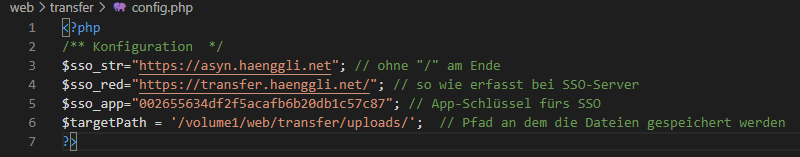
\includegraphics[width=1\linewidth]{content/images/prototyp_konfiguration.png}
    \caption{Konfigurationsmöglichkeiten des Prototyps}
    \label{fig:Konfigurationsmoeglichkeiten_prototyp}
\end{figure}
In den nächsten beiden Abschnitten werden die Gedanken zu den Konfigurationsmöglichkeiten erläutert.

\subsection{User Identifizierung}
Wie im Abschnitt \hyperref[subsec:Links]{Generierung der Links} beschrieben, dürfen Links fürs Hoch- und Herunterladen nur 
von Migratoren erstellt werden können. Dafür bedarf es eines Logins. Durch die vorgegebene Hardware ist es möglich, 
die bestehenden Benutzer des Synology NAS zu verwenden. Synology bietet eigens dafür eine Anleitung inkl. PHP- und Frontendbeispiele an \cite{Synology}.
Durch das so nutzbare Single Sign On entfällt eine zusätzliche Userverwaltung. 
So ist es einfach möglich Migratoren (=eingeloggte User) von Kunden (=nicht eingeloggte User) zu unterscheiden.
\\ 
Die nötigen Parameter für die Anbindung eins beliebigen Synology-NAS können mit den Variablen beginnend mit ``\$sso\_'' gesetzt werden.

\subsection{Datenhaltung}
Der ganze Prototyps verwaltet nur Dateien. Das ist eine Aufgabe, die das Dateisystem ebenfalls wahrnimmt.
Es ist daher sinnvoll, für die Haltung der Dateien auf das Dateisystem zurückzugreifen. 
Beim Prototyp muss daher nur angegeben werden, wo die Daten am Ende gespeichert werden sollen. 
Dies kann mit der Variable ``\$targetPath'' konfiguriert werden. 
Wird ein Pfad ausserhalb des eigentlichen WebServers hinterlegt, ist kein direkter Zugriff über eine URL auf eine Datei möglich.
Dies erhöht die Sicherheit und schützt die Daten vor unbefugten Zugriff aus dem Internet.

\clearpage
\section{Graphische Benutzeroberfläche}
Das Herzstück des Prototyps ist die Oberfläche. Diese entscheidet über gelingen oder nicht gelingen.
Wie in \cite{Butz} beschrieben, wird versucht eine möglichst einfache Oberfläche zu gestalten. Ohne verwirrende Farben oder Effekte.
Alle Links werden daher klassisch in blau gehalten. Alles andere sind nur Texte ohne dahinerliegende Aktionen.
Bei der ursprünglichen Recherche zu bestehenden Tools wurden von unzähligen Anbietern die JavaScript-Lösung DropzoneJs verwendet.
Die Dokumentation \cite{DropzoneJs} dazu ist sehr ausführlich und ebenfalls mit Serverseitigen PHP-Beispielen bestückt. 
Diese frei verfügbare Bibliothek für die Oberfläche beinhaltet die clientseitig implementierte Lösung zu zahlreichen Hürden aus den Anforderungen:
Drag\&Drop von Dateien, 
Auswahl mittels Dialogbox, 
Statusanzeige über den Stand des Hochladens,
Rückmeldungen bei Erfolg und Fehler nach dem Hochladen,
Teilung von zu grossen Dateien, 
Anstoss um Teildateien serverseitig wieder zusammenzusetzen,
Nach dem Zusammensetzen kann ein Log-Aufruf abgesetzt werden.

\begin{figure}[!h]
    \centering
    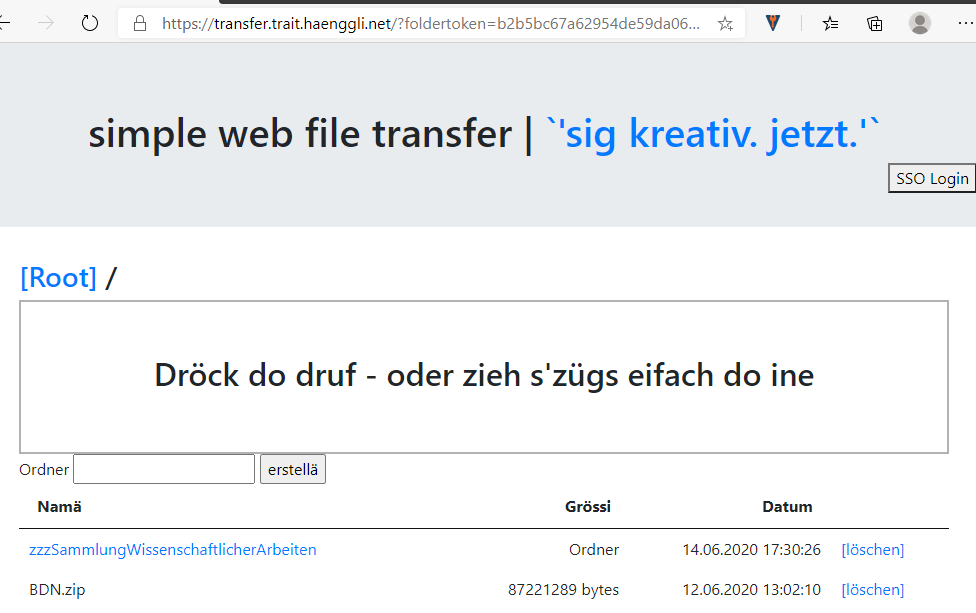
\includegraphics[width=1\linewidth]{content/images/prototyp_nichteingeloggt.png}
    \caption{Ansicht Prototyps von Kunde mittels Hochladelink}
    \label{fig:Prototyp_Hochladelink}
\end{figure}

Wie in Abbildung \ref{fig:Prototyp_Hochladelink} ersichtlich, konnte die Oberfläche sehr einfach gehalten werden.
Hochladen und Löschen sind für Kunden möglich ohne die Daten wieder einzusehen. Für die bessere Strukturierung können unbeschränkt neue Unterordner erstellt werden.
Das Synology-Loginfenster kann mit Klick auf den Button ``SSO Login'' geöffnet werden.
Einmal eingeloggt stehen weitere Möglichkeiten zur Verfügung. 

\begin{figure}[!h]
    \centering
    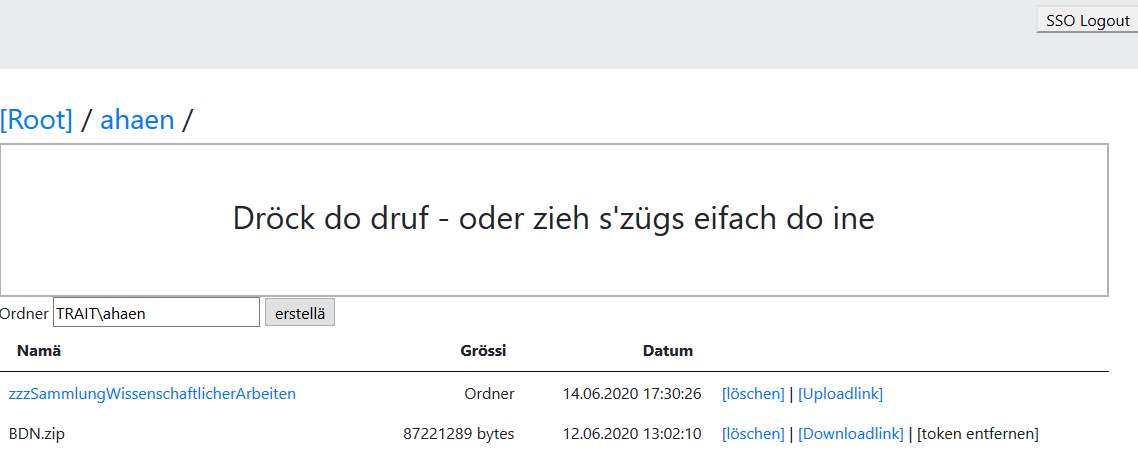
\includegraphics[width=1\linewidth]{content/images/prototyp_eingeloggt.png}
    \caption{Ansicht Prototyps nach Login}
    \label{fig:Prototyp_Migrator}
\end{figure}

Die zusätzlichen Möglichkeiten sind gemäss Abbildung \ref{fig:Prototyp_Migrator} 
die Ordnernavigation unabhängig vom Uploadlink, das erstellen weiterer Uploadlinks 
sowie das Erstellen von Downloadlinks.
Innerhalb des Netzwerk kann mit dem üblichen Dateiexplorer auf alle Dateien und Ordner zugegriffen werden.
\begin{figure}[!h]
    \centering
    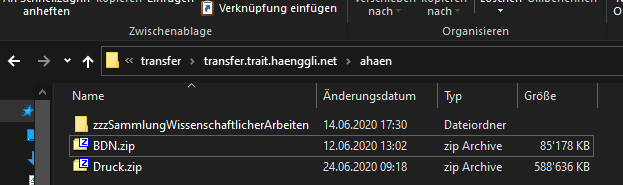
\includegraphics[width=1\linewidth]{content/images/file_explorer.png}
    \caption{Ansicht mit Dateiexplorer}
    \label{fig:file_explorer}
\end{figure}

\clearpage

Die Nutzung eines Downloadlinks ist ebenso einfach. Er kann wie eine normale Website aufgerufen werden.
Der Browser bringt dann automatisch den jeweiligen Standard Download-Dialog:
\begin{figure}[!h]
    \centering
    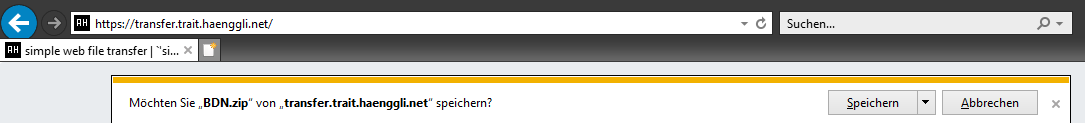
\includegraphics[width=1\linewidth]{content/images/prototyp_download.png}
    \caption{Download-Dialog im Internet Explorer}
    \label{fig:ie_download}
\end{figure}

\section{Generierung von Links}
Um die Links fürs Hochladen und Herunterladen von Dateien nicht sprechend zu gestalten, werden zufällig generierte 32stellige Werte verwendet.
Diese können durch einen Aufruf der PHP\-Funktion ``random\_bytes(32)'' erzeugt werden.
Die so erzeugten Werte werden mit dem dazugehörenden Pfad abgespeichert. Als Pfad wird der Pfad zur Datei bei Download, 
sowie der Pfad zum Ordner fürs Hochladen verwendet.
Um erneut auf eine Datenbank zu verzichten, werden die Zuweisungen ebenfalls in einer PHP-Datei gespeichert.
Durch die PHP-Endung ist der Inhalt nicht aus dem Internet ersichtlich.
\\
Nicht eingeloggte User sind nicht in der Lage neue Links zu generieren. 
Eingeloggte User können mittels Knopfdruck - wie bei Abbildung \ref{fig:Prototyp_Migrator} ersichtlich - auf ``[Uploadlink]'' klicken. 
Serverseitig wird geprüft, ob es für den Ordner bereits einen zufälligen 32stelligen Wert gibt. Falls nicht, wird einer erstellt (Abbildung \ref{fig:Srv_newLink}):
\begin{figure}[!h]
    \centering
    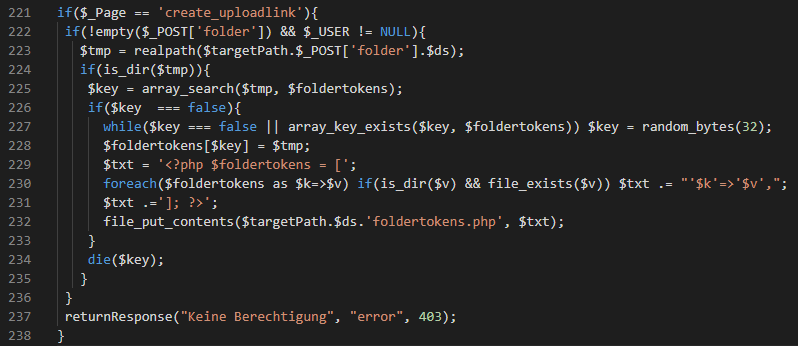
\includegraphics[width=0.9\linewidth]{content/images/prototyp_tokens.png}
    \caption{Serverseitige Generierung eines Links}
    \label{fig:Srv_newLink}
\end{figure}

\clearpage

Der so ermittelte Wert wird dann an die URL der Seite, gemäss Abbildung \ref{fig:Hochladelink_prototyp}, angehängt.
\begin{figure}[!h]
    \centering
    
\includegraphics[width=1\linewidth]{content/images/prototyp_uploadtoken.png}
    \caption{Neu generierter Hochladelink}
    \label{fig:Hochladelink_prototyp}
\end{figure}

Durch den Aufruf der Webseite mit dem URL-Parameter können die Kunden so nur die darin enthaltenen Dateien sehen. 
Ohne eine Möglichkeit diese herunterzuladen - wie bei Abbildung \ref{fig:Prototyp_Hochladelink} ersichtlich.

\section{Serverseitige Aufgaben}
Serverseitig mussten mit PHP folgende Aufgaben gelöst werden:
\begin{itemize}
    \item Kommunikation/Prüfung mit dem Synology-NAS zur Prüfung ob ein Benutzer eingeloggt ist gemäss \cite{Synology}
    \item Anbieten des Downloads bei gültigem Downloadlink
    \item Anzeige aller Ordner und Dateien anhand des Hochladelinks    
    \item Löschen von Dateien und Ordner falls ein gültiger Hochladelink verwendet wird (oder Benutzer eingeloggt ist)
    \item Loggen von hochgeladenen und heruntergeladenen Dateien für Analysezwecke
    \item Zusammensetzen von gesplitteten Dateien
    \item Falls eingeloggt: Anzeige ergänzen mit Möglichkeit Ordner zu wechseln
    \item Falls eingeloggt: Generierung von neuen Links für Hochladen und Herunterladen
\end{itemize}